\documentclass[UTF8,a4paper]{ctexart}

\usepackage{enumerate}
\usepackage{ctex,forest}
\usepackage{amsmath}

\title{Notebook of the Shipping and Shipbuilding Trading and Marketing \\
	\begin{large}
		 Memorize all of these, then you can get full marks! 
	 \end{large}}
\author{Jian}
\date{\today}

\begin{document}
	\maketitle
	\tableofcontents
	
	\section{Shipping Market Outlook}
	写在前面:凡是本文莫名其妙出现k的地方,说明是2018年的考点.
	\subsection{国际航运市场概念}
	\begin{enumerate}[*]
		\item 狭义-设在各地的航运交易所
		\item 广义-以国际航运服务的需求方作为买者,以国际航运的供给方作为卖者,以这种服务作为交换对象所组成的一种交易关系or为国际航运服务及其相关行业结合,协调,运作等活动及其关系的总和.
	\end{enumerate}
按船种分为散货船市场,油轮市场,集装箱船市场.按船舶经营范围分为东北亚市场,东南亚市场,太平洋市场,大西洋市场.按航线分为远东/欧洲航线,远东/北美航线,欧美航线.
	\begin{enumerate}[1)]
		\item 	\begin{forest}
			for tree = {grow'=east}
			[航运市场k [基本市场 
							[不定期船市场][班轮运输市场][租船市场]
							]
			   		 [相关市场(派生市场)
			   		 		[新造船市场Newbuilding Market]
			   		 		[船舶买卖市场(二手船市场)Secondhand Market]
			   		 		[拆船市场Demolition Market]
			   		 		[修船市场、船员劳务市场]
			   		 		]
			   		 ]
		\end{forest}
		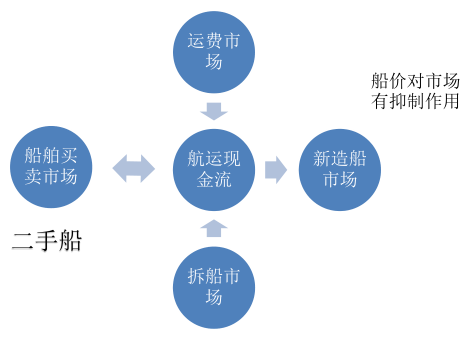
\includegraphics[scale=0.7]{cashflow}
		
		\item \begin{forest}
			[国际主要航运交易市场
								[伦敦市场]
								[纽约市场]
								[汉堡奥斯陆市场]
								[东京市场]
								[香港市场]
								]
		\end{forest}
		\item \begin{forest}
			[航交所
				[规范航运市场交易行为]
				[调节航运市场价格]
				[沟通航运市场信息]
				]
			\end{forest}
		
			上海航运交易所Shanghai Shipping Exchange 1996年11月28日
	\end{enumerate}
	\subsection{Roles}
		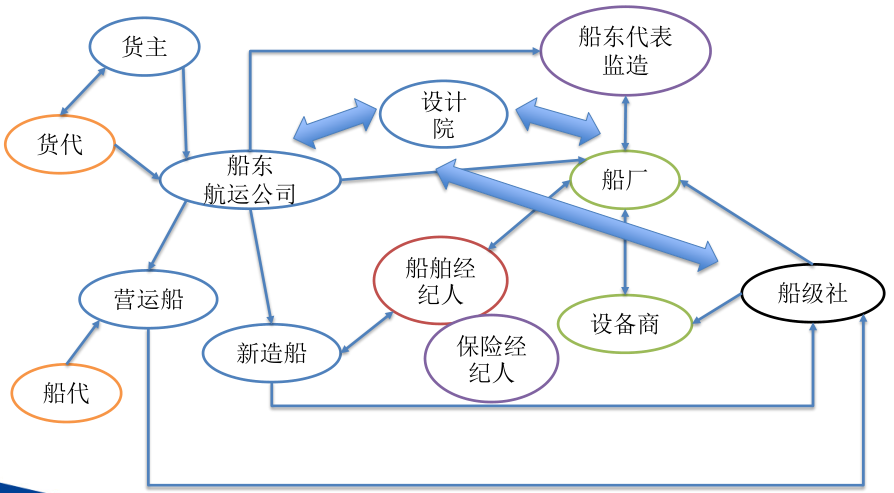
\includegraphics[scale=0.5,trim=0 0 0 0]{roles}
		船舶经纪人是专门代他人从事船舶买卖和租船业务的专业人员.分为船舶买卖经纪人和船舶货运经纪人.细分为船东,租船,通信,装货,港口,买卖经纪人.
	\subsection{国际航运基本市场}
	\begin{enumerate}[1)]
		\item 不定期船运输市场(Tramp Shipping Market)海运经营者根据海运需求在时间、地点和内容上所发生的变化,不断变更航线和货种的一种经营方式。即它没有固定的航线,港口,船期和运价。
		
		\begin{forest}
			for tree = {grow'=east}
			[主体 [供给者
					[船东
						[船舶经营者]
						[二三船东]
						]
						]
				  [需求者
				  	 [货主
				  	 	[贸易商]
				  	 	[生产商]
				  	 	[经纪人]
				  	 	[政府]
				  	 	]
				  		]
					]
		\end{forest}
	
		\begin{forest}
			for tree = {grow'=east}
			[油船k [VLCC 20-30Wton]
					[Suezmax ~15]
					[Aframax 10-12]
					[Product]
			]
		\end{forest}
		\begin{forest}
			for tree = {grow'=east}
			[干散货船
				[Capsize >10]
				[Panamax 5-7]
				[Handymax 3-5]
				[Handysize <3]
			]
		\end{forest}
			
		\begin{forest}
			for tree = {grow'=east}
				[主要货种
					[大宗干散货
						[ore]
						[煤炭]
						[粮食]
						[铝矾土]
						[磷灰石]
						]
					[小宗干散货
						[农产品]
						[木材]
						[水泥]
						[废钢铁]
						[肥料]
						]
					[液体散货
						[原油]
						[成品油]
						[液化燃气]
						[石油化工产品]
						]
				]
		\end{forest}

		\item 班轮运输市场(Liner Shipping Market)船舶按照规定的时间表,在一定航线上,以既定的挂靠港口顺序经常地从事航线上各港间的船舶运输
		
		四定:定船期,定航线,定港口,定费率
		
		\begin{forest}
			for tree = {grow'=east}
			[船舶类型
				[传统杂货船Conventional general cargo ship]
				[集装箱船Container ship]
				[滚装船Ro/Ro]
				[载驳船Barge carrier]
				[冷藏船Refrigerated ship]
			]
		\end{forest}
		
		班轮公司排名:丹麦MAERSK,瑞士地中海,法国达飞,中远海运
		
		\item 租船市场(Ship Charter Market) 以船舶运输服务或船舶的使用为对象的船东与承租人之间的交易关系
		
		租船业务是船东将船舶出租给承租人使用的一种航运业务
		
			\begin{enumerate}[a)]
				\item 租船市场比不定期运输市场范围大.不定期船运输$=$租船运输(货主向船东租船或船东出租船给货主).而租船市场$=$租船运输$+$船东与船舶经营者之间的租船
				\item 
					\begin{forest}
						for tree = {grow'=east}
						[租船形式k
							[航次租船Voyage Charter]
							[定期租船Time Charter]
							[包运租船COA-Contract of Affreightment]
							[光租船Demise Charter/Bareboat Charter]
							[航次期租TCT-Trip Charter on Trip Base]
							]
					\end{forest}
				\item 租船市场的作用
					\begin{enumerate}[.]
						\item 专门为船东和租船人提供各种租船业务机会
						\item 租船市场快速有效地为船东和租船人成交租船业务
						\item 调节世界航运市场
						\item 为船东和租船人提供大量的租船市场信息,资料等行情动态,发展趋势
					\end{enumerate}
			\end{enumerate}
		
		\item 航运供需关系分析 (课件中的工程船是什么意思)
		\begin{enumerate}[.]
			\item 航运需求市场
				\begin{enumerate}[-]
					\item 运输对象的空间位移服务
					\item 与贸易量,装港和卸港的地理位置和距离有关
					\item 三个全球化发展阶段
				\end{enumerate}
			国际贸易是航运市场需求的来源,全球化是驱动海运发展最重要的因素.按国际贸易商品的自然特性不同,分为散货运输和班轮运输.
			\item 航运供给市场
				-吨位,船舶使用效率(待时,亏载,空驶),航速
				
				-属性:大宗商品,周期滞后,长周期,产业转移
			\item 造船业投资特点k
				(航运业是一项投资额巨大,投资回报周期长,经营风险大的行业.船舶融资指船舶业中的经济主体融通和筹措船舶投资资金的行为和活动.融资方式:商业银行贷款,出口信贷,融资租赁,债券市场融资,股票市场融资.)
				\begin{enumerate}
					\item 随市场波动,量价同时变化
					\item 长周期
					\item 周期滞后
					\item 产业转移
				\end{enumerate}
			\item 特征
				\begin{enumerate}
					\item 周期性5-15年
					\item 季节性 仅航运市场
					\item 不规则偶发性 战争/石油危机
					\item 长期趋势 对船舶安全,舒适性和环保的要求,双壳油轮,油舱隔离
				\end{enumerate}
		\end{enumerate}
	
	\item 航运市场分析
		1)国际波罗的海综合运费指数BDI:Capesize,Panamax及Handysize权重均分.因散装航运业营运状况与全球经济景气荣枯、原物料行情高低息息相关,故波罗的海指数可视为经济领先指标。
		
		2)克拉克森海运运价指数
	\end{enumerate}
	
	\subsection{国际航运相关市场}
		\begin{enumerate}[1)]
			\item 新造船市场:船主与造船厂之间以建造新船为对象而形成的交易关系
			反映造船业景气度的三大指标:造船完工量,新接订单量,手持订单量.
				\begin{enumerate}[.]
					\item 造船市场与航运市场的关系
						
						-造是航供给的主要来源
						
						-造的订造量的增减迟于航的变化
						
					\item 基本特征
						\begin{enumerate}[-]
							\item 不可取代
							\item 不稳定
							\item 国际合作
							\item 船舶单价昂贵
							\item 造船周期长
							\item 合同预定
						\end{enumerate}
					\item 新造船市场的影响因素
						\begin{enumerate}[-]
							\item 世界经济与国际贸易
							\item 货运结构
							\item 国际公约
							\item 航运政策
							\item 人为因素
							\item 国际金融与汇率
							\item 战争
						\end{enumerate}
					\item 新造船舶价格的影响因素
						\begin{enumerate}[-]
							\item 航运市场的运价水平
							\item 对航运市场未来趋势的预测
							\item 国际信贷的优惠程度
							\item 造船能力的利用程度
							\item 造船成本
							\item 所订造船舶的技术和设备要求
						\end{enumerate}
					\item 规律
						\begin{enumerate}[-]
							\item 航运市场景气$->$新造船舶需求增加$->$船价up
							\item 船价低,贷款条件优惠?$->$航运市场萧条$->$运输需求最低
							\item 如何利用航运市场与新造船市场的矛盾?
						\end{enumerate}
				\end{enumerate}

			
			\item 买卖市场:买主与卖主之间以二手船(旧船)为交易对象而形成的交易关系
			好处:投资额少,可立即投入生产运营,性能易于掌握.
				\begin{enumerate}[.]
					\item 二手船与新船的比较
					\item 影响船舶买卖市场价格的主要因素
						\begin{enumerate}[-]
							\item 当前航运市场的行情
							\item 对航运市场未来行情的估计
							\item 新船价格
							\item 船舶的技术状况
							\item 船舶附带的期租合同
						\end{enumerate}
				\end{enumerate}
			
			\item 拆船市场:船主与拆船业之间以拆卸旧船为对象而形成的交易关系,是减少航运市场运力供给的主要途径.
			
			影响拆船价格的因素:船的种类和陈旧程度,交易方式,船的状态
			
			影响拆船数量的因素:船舶市场提供的废船数量,钢铁工业对拆船钢料的需求,废船交船地的地理位置,废船交易的季节性(台风)
		\end{enumerate}
	
		\subsection{其他部门}			
			 港务局,海事局(MSA)
			 
			 船级社k(Classification Society)是一个建立和维护船舶和离岸设施的建造和操作的相关技术标准的机构.登记的民间组织.主要业务:对新造船舶进行技术检验,合格者给予船舶的各项安全设施并授给相应证书;制定技术规范和标准.日本海事协会NK,英国劳氏船级社LR,挪威船级社DNV与德国劳氏船级社GL合并,美国船级社ABS,中国船级社CCS,韩国船级社KR.
		\subsection{方便旗}
			 Flag of Convenience表明国籍,在公海上受船旗国的专属管辖和保护.无国籍的船舶在公海上被认为是海盗船.船舶登记手续简化,登记费低,船舶吨税和检查费用低. 重要!国旗记一下
			 \begin{figure}
			 \centering
			 
\includegraphics[scale=0.2,trim=0 0 0 0]{antigua}
			 \caption{安提瓜和巴布达}
			 
\includegraphics[scale=0.1,trim=0 0 0 0]{liberia}
			 \caption{利比里亚}
		   		
\includegraphics[scale=0.5,trim=0 0 0 0]{marshall}
		   		\caption{马绍尔群岛}
		   		
\includegraphics[scale=0.3,trim=0 0 0 0]{panama}
		   		\caption{巴拿马}
		   	\end{figure}
		\subsection{国际贸易术语k}
			\begin{enumerate}[.]
				\item FOB Free on Board 指定装运港船上交货 FOB Under Tackle(FOB吊钩下交货)指卖方负担费用将货物交到买方指定船只的吊钩所及之处,而吊装入舱及其他各项费用概由买方负责.
				\item CIF Cost Insurance and Freight 成本加运费保险费
				\item CFR/CNF Cost and Freight 成本加运费
				\item L/C Letter of Credit 信用证
				
			\end{enumerate}

		
	\section{船舶建造工程报价}
		\subsection{报价的原则和程序!}
			\begin{enumerate}[1)]
				\item 报价与询价
					
					询价(一般征询,具体询盘)
					\begin{enumerate}[-]
						\item 询价内容,见课本
						\item 询价要求
						\item 催询
						\item 研究报价
					\end{enumerate}
				
					报价
					\begin{enumerate}[-]
						\item 报价的重要性和竞争性
						\item 报价的原则 
							
						\item 关于报价的价格水平问题 了解
					\end{enumerate}		
				
				\item 造船报价!
					船价及其依据:虚盘-基本参数,如$L_{OA}, B, D, T, \delta$等,实盘-报价附有简要规格书及总布置图.
					
					报价项目:船价中已包括及未包括的项目.
					\begin{enumerate}[.]
						\item 付款!
							\begin{enumerate}[-]
								\item 付款期数
									\begin{enumerate}[.]
										\item 签订合同
										\item 铺龙骨(下料,上船台)
										\item 下水
										\item 交船
									\end{enumerate}
								\item 每阶段付款所占合同总价比例
							\end{enumerate}
						\item  财务安排:延迟付款,信贷
						\item 买方提供的项目和内容
						\item 报价有效期
					\end{enumerate}
				\item 报价机构和报价人员 了解
				\item 报价前的准备工作
				\item 造价动态成本观念 报价$=$物料支出$+$劳动力报酬$+$盈利
			\end{enumerate}	
	
	\section{船舶经济指标及分析}
		货币的时间价值:绝对方式--利息(单利,复利);相对方式--利率.
		
		终值是本金按照给定利率在若干计息期后按复利计算的本利和.终值与复利是一对对应的概念.
		
		现值是未来的资金按照一定利率折算而成的当前价值.折算过程称为贴现.贴现现金流量法DCF.$P=F\cdot(1+i)^{-n}$
		现金流量图!
		
		资金等值:一定数量的资金在不同时间代表不同的价值.影响因素:金额大小,发生时间,利率
		
		名义利率:给定年利率(名义利率$i_{nom}$/APR),若在一年内计算复利,则必须用$i_{nom}$除以每年内的计息次数m得到期利率$i_{per}$,根据实际利息与本金之比算的的利率称为有效利率/实际利率Effective Annual Rate--EAR
		
		$EAR=(1+\frac{i_{nom}}{m})^m-1=(1+i_{per})^m-1$
		
		离散复利$F=p\cdot(1+i)^n$
		
		离散贴现$P=F\cdot(1+i)^{-n}$
		
		连续复利$F=P\cdot e^{in}$
		
		连续贴现$P=F\cdot e^{-in}$
		
		例题P->A k!
		
		资金时间价值:
		
		终值因数
		
		现值因数
		
		等额终值因数
		
		等额预付因数
		
		等额现值因数
		
		资金回收因数
		
		
		指标 k!
		\begin{enumerate}[$\cdot$]
			\item 净现值Net Present Value
			
			NPV各年收入和支出,按基准折现率折现后相减的差值.表示盈利.衡量经营者的满意度,RFR是使船东的顾客满意的最低标准. 
			
					$NPV=-P + (B-Y)\frac{1-(1+i)^{-N}}{i}+L(1+i)^{-N}$ 
					
				方案投资额不等时,NPV偏向于大投资额(绝对盈利大),NPVI(相对数额).方案寿命期不等时,NPV偏向寿命长的.AAC偏向短的.
				
			\item 内部收益率Internal Rate of Return important!
		
			IRR船舶使用期内使NPV=0的投资收益率.表示方案负担得起的贷款利率,大了好.
			
			\item 平均年费用Average Annual Cost 
			
			AAC将投资的现值用复利计算平摊到每年,再加上每年平均的营运费用.直观反应每年开支,适用于无需考虑收入的方案.
			
				$AAC = (P-L)\frac{i}{1-(1+i)^{-N}}+Li+Y$
			
			\item 必要运费率Required Freight Rate RFR为达到预定的投资基准收益率,单位运量最低限度所需要的收入,兼顾托运方和船方的利益,适用于收入不能预估的方案.
				$RFR=\frac{AAC}{Q}$ important!
		\end{enumerate}
	
	\section{船舶造价估算}
		\subsection{成本组成 k!}
		\begin{forest}
			for tree = {grow'=east}
			[Cost [原材料26-33\%]
					[配套设备45-52
						[直接购入]
						[间接购入]
						]
					[劳务费24-26
						[工人直接工资]
						[工人间接工资]
						]
					[管理费
						[企业管理费]
						[others]
						]
				]
		\end{forest}
	
		\subsection{造船成本的估算方法k}
			\begin{enumerate}
				\item 方案设计研究阶段$cost=$船体工程费用+轮机+舾装+电气+专用费用
			\end{enumerate}
		
		\subsection{船舶设计参数变化对建造成本的影响}
		载重量,主尺度,航速. 载重量的变化可视为主尺度的变化,同时也必将导致船的建造成本的变化.
		
		批量生产对船舶成本的影响!
			\begin{enumerate}[$\cdot$]
				\item 经验曲线
				\item $\overline{Y_x}=\frac{a}{X^b}$
				\item $\lambda=\frac{1}{2^b}$最低反应批量经济效益最好
			\end{enumerate}
		
	\section{船舶招投标及实务}
		\begin{forest}
			for tree = {grow'=east}
			[招标方式!
					[竞争性招标ICB
						[公开招标Open bidding]
						[选择性招标Selected bidding]
					]
				[谈判招标]
				[两段招标:结合无限竞争招标和有限竞争招标]
				]
		\end{forest}
	
		
		流程k
		
		发招标通告-资格预审-编制投标书-编制投标书并落实担保-递送投标文件-开标-评标和决标-中标签约-end
		
		招标书
		
		投标 购买标书? 商务标书:报价,针对打分条款的回应;技术标书:如何取做该项目,质量,进度,成本控制.
		
		实务 案例; 研究标书,资质,标的,特殊设备,评分细则等; 标书文件制作; 投标时间; 开标.
		
	\section{二手船买卖标准合同}
		船舶买卖流程:
		
		1.达成买卖合约(1.卖方经纪人:发出询购意向;2.买方经纪人发出第一个要约;3.卖方在要约规定答复时限内回实盘;4.经纪人起草一份双方谈判内容的完整重复Recap); 
		
		2.买方支付保证金(10percent);
		
		3.买方检查船级社记录与上船检查(NSF93 2); 
		
		4.买方检查船级社纪录与上船检查(NSF93 4); 
		
		5.买方派代表/船员上船熟悉操作(15);
		
		6.卖方准备交船工作k;
		
		7.买方准备接船工作;
		
		8.蛙人进干坞检查水下部分;
		
		9.卖方递交通知书;
		
		10.买卖双方准备交接(实质交接和法律交接);
		
		11.买方接船后的工作.
		\begin{forest}
			for tree = {grow'=east}
			[,phantom
				[主要人员
					[买卖双方]
					[双方经纪人]
					[双方银行]
					]
				[其他人员
					[双方律师]
					[船级社]
					[船舶注册国的海事机构]
					]
				]
		\end{forest}
	
	\section{somebody's ppt}
		\subsection{市场结构k}
			定义!
			研究意义:通过不同市场结构中追求利润最大化的厂商行为及其结果的分析,认识市场机制在有效配置经济资源中的作用.市场结构-行为-绩效.厂商行为方式与厂商所处市场结构状况有关.市场绩效是指市场结构(机制)在使供给者对稀缺资源的配置使消费者获得最大利益的情况.
			
			市场结构划分的依据:市场中买者与卖者的数目;商品的差别;市场进入和退出的难易程度;单个厂商对市场价格的控制能力;信息的完备性.
		\subsection{Shipping Cycle}
			航运周期成因:
				\begin{enumerate}[1)]
					\item 外因论:经济周期的根源在于市场经济体制之外的某些事物的波动.
						\begin{enumerate}[.]
							\item 太阳黑子->气候->农业收成->经济 10years
							\item 科技的创新无法一直出现,创新使一种新的生产函数
							\item 政府的周期性决策(循环解决通货膨胀和失业问题)
						\end{enumerate}
					\item 内因论:市场经济体制本身因素相互制约和促进的运行机制
						\begin{enumerate}[.]
							\item 纯货币理论:货币供应量and流通度,短期利率
							\item 投资过度:资本品生产的过度发展使经济繁荣,过剩又使经济萧条
							\item 消费不足
							\item 心理
						\end{enumerate}
				\end{enumerate}
			航运市场周期
			60年长周期,反映了世界经济发展,不受船业控制,顶峰由主要科技进步导致,低谷由主要危机,如饥荒战争导致.
			5-10年短周期,主要由船市商业运营导致.有四个阶段k
				\begin{enumerate}[(1)]
					\item Trough:过剩,运费跌至白菜价(最烂的船能漂着的成本),银行变大爷公司变孙子.
					\item Recovery:供应量跌得靠近需求量,触底反弹了要,市场情绪难以揣摩但在变自信.
					\item Peak:旧船说扔就扔,大量订单船厂乐开怀,拆船量少,银行变孙子.
					\item Collapse:Heavy ordering->huge delivery->overcapacity,运价跳水,祸不单行,船慢,人们不愿相信一个土匪的名字叫牧之.
				\end{enumerate}
			
			季节性明显,运价和季节息息相关.
			
			我们处于Recovery阶段.
			
			前车之鉴:船市周期7-8年,每个轮回都不一样.船业高危,控制需求是不可能的,只能调节供给来维持稳定运价,我们能做的只有提供更好的信息,改善分析和预测.轮回就是命,跳不出的.
			
			Conclusions:船市周期有不同的成分,短周期的作用是调节船市的供需平衡,有四个阶段.这些阶段是偶发性的,时间没有特定规律,预测阶段是不可能的,这辈子也不可能预测下一个周期.
			
	\section{Complementary}
		
		价格是否是投标过程中的决定因素?如何防止恶意低价中标?k
	
		
		船价估算.新造船,二手船市场特点,造船业投资/二手船废船交易特点,国际贸易术语.经济指标,计算题.船级社基本特征.二手船租船.NFS93合同基本条款和说明.招标流程.
\end{document}